\section{Application: cadmium concentrations in the Swiss Jura}
\label{sec:application}
\subsection{Data and prediction task}
The Jura soil survey measured trace-metal concentrations across a 14.5-km$^2$ area near La Chaux-de-Fonds, Switzerland \citep{atteia1994jura}. We use the 359-site dataset documented by \citet{goovaerts1997geostatistics} and distributed with \texttt{gstat} \citep{pebesma2004gstat}. The response is the natural logarithm of cadmium concentration, originally measured in mg/kg of topsoil. We retain the dataset's original split into 259 training sites and 100 reserved validation sites (Figure~\ref{fig:application}A). These reserved sites define our prediction target, with equal weights. Their measured concentrations allow a direct comparison between CV estimates and observed target MSE: the average squared prediction error at the 100 sites, on the log scale.

Ordinary kriging predicts log-cadmium using an estimated constant mean, exponential covariance and a nugget. Mean and covariance parameters are re-estimated using only the training observations available within each CV fold. A separate fit to all 259 training observations supplies the final prediction model. Target concentrations enter only the evaluation of its predictions.

\subsection{CV schemes and evaluation}
We compare the four five-fold schemes in Section~\ref{sec:cv-selection}: random folds, coordinate blocks, buffered blocks and kNNDM. The buffer is the median nearest-other-training distance. For this split, it removes no additional observations from the block training sets, so these two candidates coincide. We repeat fold construction 40 times with different random seeds. The training and target data and the final fitted model stay fixed. kNNDM returns the same folds every time.

We select the scheme with the smallest $W$ or $|J_2|$ and compare its CV score with observed target MSE at the 100 reserved sites. All candidates use the same full-training covariance estimate for $J_2$. The 40 repetitions describe variation due to fold allocation within this survey. The supplementary material (Section~\ref*{supp-sec:jura-fitting}) describes covariance estimation.

\subsection{Results and interpretation}
For the original 100 validation sites, random CV gives a closer estimate of observed target MSE than kNNDM. The observed target MSE is \JuraPublishedTarget: random CV averages \JuraPublishedRandomScore, whereas kNNDM gives \JuraPublishedKnnScore\ (Figure~\ref{fig:application}E). Random CV therefore underestimates the measured prediction error, while kNNDM overestimates it. Across the 40 repetitions, the mean absolute difference from observed target MSE is \JuraPublishedRandomMAE\ for random CV and \JuraPublishedKnnMAE\ for kNNDM. Both block schemes overestimate more strongly, averaging \JuraPublishedBlockScore.

Both diagnostic rules nevertheless select kNNDM in every repetition. Its validation distances most closely match the target distances (Figure~\ref{fig:application}B), and it has the smallest $W$ and $|J_2|$ (Figure~\ref{fig:application}C--D). Thus, the scheme that best matches these nearest-neighbour summaries does not give the most accurate CV estimate for this dataset.

The comparison changes when the target is the 100 northernmost sites. Both rules then select the block schemes, whose mean absolute difference from observed target MSE is \JuraNorthBlockMAE, compared with \JuraNorthRandomMAE\ for random CV. Adding a linear coordinate trend leaves these conclusions unchanged. The supplementary material (Section~\ref*{supp-sec:jura-sensitivity}, Table~\ref*{supp-tab:jura-selection} and Figure~\ref*{supp-fig:jura-targets}) reports these checks and the random-holdout comparison.

\begin{figure}[p]
\centering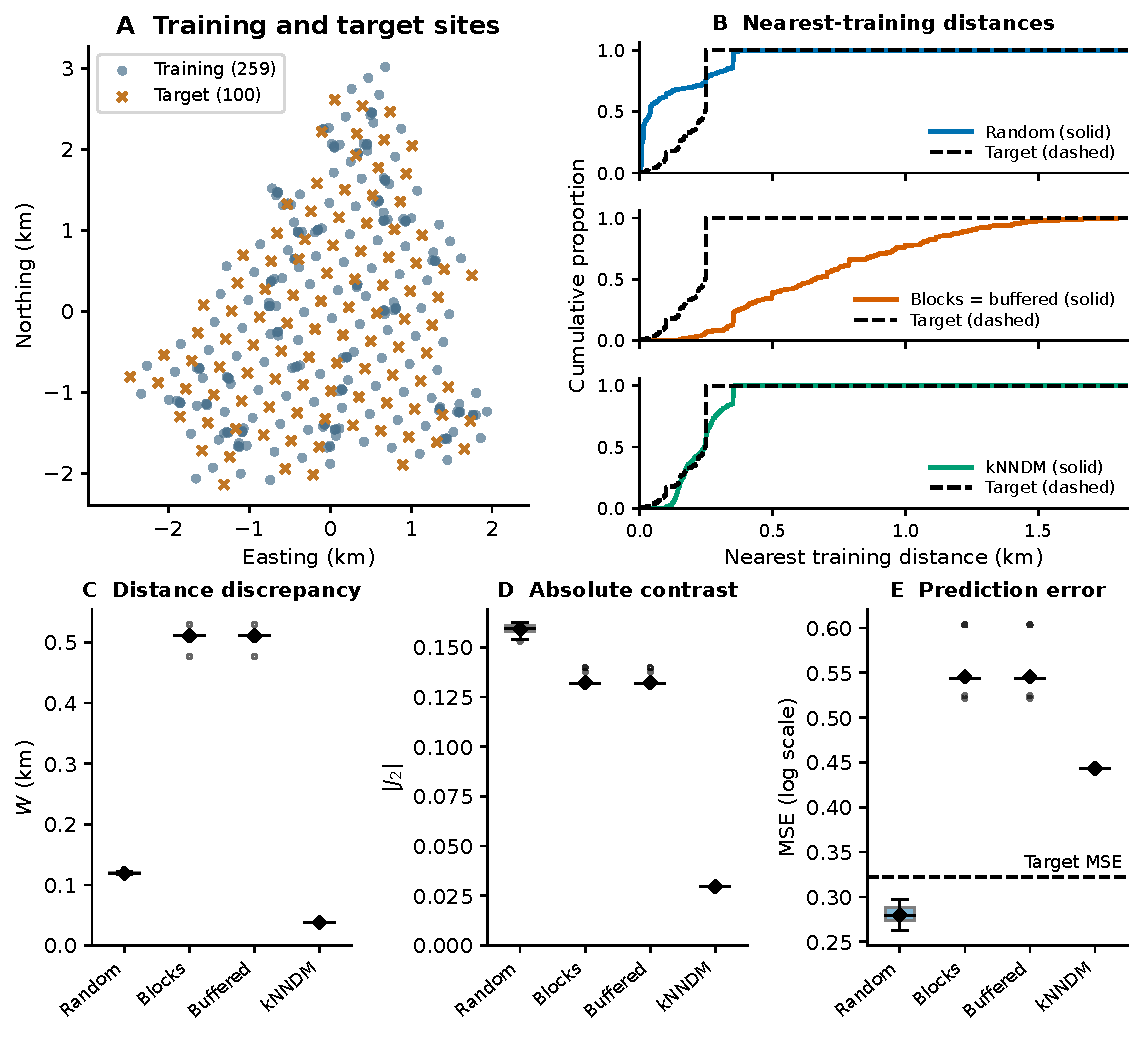
\includegraphics[width=\textwidth]{F4-application.pdf}
\caption{CV selection and observed prediction error for log-cadmium in the Swiss Jura. (A) The 259 training sites and 100 reserved target sites; coordinates are relative to the training-site centre. (B) In each comparison, the solid curve gives the proportion of validation sites with a nearest training neighbour within the indicated distance. The dashed curve gives the corresponding proportion for target sites. All three comparisons use the same axes and repetition 1; blocks and buffered blocks coincide. (C--D) $W$ and $|J_2|$: each rule selects the scheme with the smallest value. (E) CV MSE compared with observed target MSE (dashed line). In C--E, diamonds show means over 40 fold constructions, boxes show medians and interquartile ranges, and whiskers extend to observations within 1.5 interquartile ranges; points beyond them are shown separately. kNNDM gives identical values throughout. All MSEs use natural-log cadmium.}
\label{fig:application}
\end{figure}
